% ============================================================================
% Handbuch Semera Workshops
%
% Übersetzen mit (zweimal, damit Inhaltsverzeichnis und Verweise stimmen):
%     pdflatex manual.tex
%
% Die Bilder liegen im Ordner manual_images/ neben dieser Datei.
% Mit "% NEU" markierte Stellen sind Ergänzungen gegenüber manual.docx,
% mit "% GEÄNDERT" Stellen, die gegenüber manual.docx angepasst wurden.
% ============================================================================
\documentclass[a4paper,11pt]{article}

\usepackage{iftex}
% pdfLaTeX: T1-Schrift; XeLaTeX/LuaLaTeX: fontspec. Mit T1 unter XeLaTeX wird "ß" als "SS" gesetzt.
\ifPDFTeX
\usepackage[utf8]{inputenc}
\usepackage[T1]{fontenc}
\usepackage{lmodern}
\else
\usepackage{fontspec}
\fi
\usepackage[ngerman]{babel}
\usepackage[a4paper,left=2.5cm,right=2.5cm,top=2.5cm,bottom=2.2cm]{geometry}
\usepackage{graphicx}
\usepackage{fancyvrb}
\usepackage{enumitem}
\usepackage{fancyhdr}
\usepackage{longtable}
\usepackage{booktabs}
\usepackage{array}
\usepackage[hyphens]{url}   % lange Web-Adressen dürfen auch an Bindestrichen umbrochen werden
\usepackage[hidelinks]{hyperref}

\newcommand{\manualversion}{2.0.0}
\newcommand{\manualdate}{24.10.2026}

\graphicspath{{manual_images/}}

\setlength{\parindent}{0pt}
\setlength{\parskip}{0.6em}
\setlist{itemsep=0.2em,topsep=0.3em}

\pagestyle{fancy}
\fancyhf{}
\setlength{\headheight}{14pt}
\fancyhead[L]{Handbuch Semera Workshops -- V\manualversion}
\fancyhead[R]{\manualdate}
\fancyfoot[C]{\thepage}

% Bilder stehen am rechten Rand, in der Größe wie im Word-Dokument (höchstens so breit wie der Text).
\newlength{\imgw}

% Breites Bild allein: rechtsbündig in eigener Zeile (daneben ist kein Platz für Text).
\newcommand{\bild}[2]{%
\par\smallskip\noindent
\setlength{\imgw}{#1in}%
\ifdim\imgw>\linewidth\setlength{\imgw}{\linewidth}\fi
\hfill\includegraphics[width=\imgw]{#2}\par\smallskip}

% Text links, Bild rechts: \begin{mitbild}{Breite in Zoll}{Datei} ... Text ... \end{mitbild}
\newlength{\mbtext}
\newlength{\mbpic}
\newenvironment{mitbild}[2]{%
\def\mbfile{#2}%
\par\medskip\noindent
\setlength{\mbpic}{#1in}%
\setlength{\mbtext}{\linewidth}%
\addtolength{\mbtext}{-\mbpic}%
\addtolength{\mbtext}{-1.5em}%
\minipage[t]{\mbtext}%
\vspace{0pt}\vspace{-\parskip}\sloppy
}{%
\endminipage\hfill
\minipage[t]{\mbpic}%
\vspace{0pt}\includegraphics[width=\mbpic]{\mbfile}%
\endminipage\par\medskip}

\newcommand{\pfeil}{\ensuremath{\rightarrow}}

\begin{document}

\begin{center}
  {\LARGE\bfseries Handbuch Semera Workshops}\\[0.6em]
  Version \manualversion{} -- Stand: \manualdate
\end{center}

\tableofcontents
\newpage
Vor der ersten Benutzung bitte die Workshops hinzufügen und eine Teilnehmenden-Liste importieren!

Das Importieren der Teilnehmenden ist für die Funktion der App nicht notwendig, aber sehr hilfreich.

Es ist zwingend notwendig die Workshops zu pflegen, wenn man diese nicht importieren möchte, kann man über die „Workshops bearbeiten“-Funktion auch die Workshops direkt hinzufügen.

% NEU
\section{Neuerungen in dieser Version}\label{sec:neuerungen}

\begin{itemize}
  \item \textbf{Excel-Import und -Export} für Präferenzen, Workshops und Teilnehmer, mit Zuordnung der Spalten
  (Abschnitte~\ref{sec:importdialog} und~\ref{sec:exportdialog}).
  \item \textbf{Zuteilung als Excel-Datei} speichern (Menü \emph{Zuteilungen} \pfeil{} \emph{Zuteilung speichern}).
  \item \textbf{Auswertung} rechts im Hauptfenster: Wie viele Personen haben ihre 1.~Wahl bekommen, wer ist noch nicht
  zugeteilt, wie viele Plätze sind frei (Abschnitt~\ref{sec:auswertung}).
  \item \textbf{Durchläufe}: Die Zuteilung kann mehrfach durchgeführt werden, übernommen wird der Durchlauf mit den
  meisten ersten Wahlen (Abschnitt~\ref{sec:durchlaeufe}).
  \item Bis zu \textbf{7 Tage} und bis zu \textbf{7 Wünsche}.
  \item \textbf{Händisch zuweisen} per Rechtsklick, bei mehreren Tagen für jeden Tag einzeln
  (Abschnitt~\ref{sec:haendisch}). Wer in seinen Wünschen keinen Platz bekommt, wird nicht mehr zufällig verteilt,
  sondern bleibt offen.
  \item \textbf{QR-Code}: Auswahl des richtigen Netzwerks, die Adresse für iPhones (\texttt{semera.local}) funktioniert
  jetzt (Abschnitt~\ref{sec:qr}).
  \item Die \textbf{Teilnehmeransicht} lädt deutlich schneller und kommt besser mit schlechtem WLAN zurecht
  (Abschnitt~\ref{sec:teilnehmeransicht}).
  \item Neuer Abschnitt \textbf{Netzwerk und Router} mit den nötigen Router-Einstellungen, einer festen IP-Adresse und
  gedruckten QR-Codes (Abschnitt~\ref{sec:netzwerk}).
  \item Verwaltung, Import, Löschen und Zuteilen sind aus Sicherheitsgründen nur noch an dem Rechner möglich, auf dem das
  Programm läuft.
\end{itemize}

\section{Präferenz-Verwaltung}\label{sec:praeferenzen}

\begin{mitbild}{2.04}{image1.jpeg}
  Hier können die \textbf{Workshop-Wahlen} der Teilnehmenden eingesehen, bearbeitet und verwaltet werden.

  \begin{itemize}
    % GEÄNDERT
    \item \textbf{Export} \pfeil{} Öffnet einen Dialog: Die Workshop-Wahlen können als Excel-Datei (\texttt{.xlsx}) oder im
    \texttt{.json}-Format exportiert werden (Abschnitt~\ref{sec:exportdialog}).
    \item \textbf{Import} \pfeil{} Importiert Workshop-Wahlen aus einer Excel-Datei (\texttt{.xlsx}), einer CSV-Datei oder im
    \texttt{.json}-Format. Welche Spalte welche Daten enthält, kann im Dialog festgelegt werden
    (Abschnitt~\ref{sec:importdialog}).
  \end{itemize}

  \textbf{Beispiel-Datei} (\texttt{preferences.json}):
  \begin{Verbatim}[frame=single,fontsize=\small]
[
  {
    "id": 1,
    "name": "Max Mustermann",
    "preferences": {
      "first": "Workshop A",
      "second": "Workshop B",
      "third": "Workshop C"
    }
  },
  {
    "id": 2,
    "name": "Erika Musterfrau",
    "preferences": {
      "first": "Workshop B",
      "second": "Workshop A",
      "third": "Workshop D"
    }
  }
]
  \end{Verbatim}

  % NEU
  In der Datei stehen die Wünsche unter \texttt{first}, \texttt{second}, \texttt{third} usw. bis \texttt{seventh}
  (so viele, wie in den Einstellungen festgelegt sind).
\end{mitbild}

\textbf{Tabelle:}\par\nopagebreak
\bild{6.38}{image2.jpeg}

\begin{itemize}
  % GEÄNDERT
  \item Spalten: \textbf{Name, Erste Wahl bis Siebte Wahl, Aktionen} (es erscheinen so viele Wahl-Spalten, wie in den
  Einstellungen festgelegt sind)
  \item In der \textbf{Aktionsspalte} können Einträge gelöscht werden.
  \item \textbf{Rote Markierung:} Falls kein Teilnehmer gefunden wird. Dieses Feature ist dafür gedacht, um zu überprüfen ob eine Person ihren Namen falsch geschrieben hat. Der eingetragene Name wird genau so wie er in der Liste angezeigt wird auch direkt ausgedruckt. Die Zeile wird also Rot markiert, falls die Abgabe nicht mit den erwarteten Namen übereinstimmt.
  \bild{5.91}{image3.jpeg}
  \item \textbf{Grüne Markierung:} Diese zeigt nach einer generierten Zuteilung an, welcher Wunsch für eine Person gewählt wurde.
  % NEU
  Bei einer Zuteilung über mehrere Tage steht in der grünen Zelle zusätzlich eine \textbf{kleine Zahl}: der Tag, an dem
  dieser Wunsch zugeteilt wurde.
  \bild{5.57}{image4.png}
  % GEÄNDERT
  \item \textbf{Personen können händisch per Rechts-Klick zugewiesen werden.} Ein Rechtsklick auf einen Namen oder einen
  Wunsch öffnet das Menü zum Zuweisen (Abschnitt~\ref{sec:haendisch}).
\end{itemize}

\subsection*{Bearbeiten per Doppelklick}

\begin{itemize}
  \item Name oder eine Wahl doppelt anklicken \ensuremath{\rightarrow} direkt editierbar.
  % GEÄNDERT
  \item Änderungen werden \textbf{automatisch gespeichert}. \pfeil{} Beim Speichern werden überflüssige Leerzeichen am Rand
  und doppelte Leerzeichen entfernt, und ein Workshop-Name wird in der Schreibweise des vorhandenen Workshops
  gespeichert (Groß- und Kleinschreibung spielt dabei keine Rolle). Tippfehler im Namen eines Workshops werden dagegen
  nicht erkannt, dann passt der Wunsch zu keinem Workshop und wird bei der Zuteilung ignoriert.
  \item Ein Name kann nur \textbf{einmal} vorkommen (Groß- und Kleinschreibung wird nicht unterschieden). Benennt man
  einen Eintrag so um, dass der Name schon vergeben ist, erscheint eine Meldung und die Änderung wird nicht
  gespeichert.
\end{itemize}

\subsection*{Zeilen löschen}

\begin{itemize}
  \item Besonders sinnvoll, wenn es \textbf{Doppel-Einträge} gibt.
\end{itemize}

\section{Workshops verwalten}\label{sec:workshops}

\begin{mitbild}{2.04}{image5.jpeg}
  Hier können die \textbf{Workshops} eingesehen, bearbeitet und verwaltet werden.

  \begin{itemize}
    % GEÄNDERT
    \item \textbf{Export} \pfeil{} Öffnet einen Dialog: Die Workshops können als Excel-Datei (\texttt{.xlsx}) oder im
    \texttt{.json}-Format exportiert werden (Abschnitt~\ref{sec:exportdialog}).
    \item \textbf{Import} \pfeil{} Importiert Workshops aus einer Excel-Datei (\texttt{.xlsx}), einer CSV-Datei oder im
    \texttt{.json}-Format (Abschnitt~\ref{sec:importdialog}). Beim Import werden die vorhandenen Workshops ersetzt oder die
    neuen angehängt, je nach Auswahl im Dialog.
  \end{itemize}

  \textbf{Beispiel-Datei} (\texttt{workshops.json}):
  \begin{Verbatim}[frame=single,fontsize=\small]
[
  {
    "id": 1,
    "title": "Workshop A",
    "maxParticipants": 20,
    "minParticipants": 5,
    "staff": "Herr Schmidt",
    "location": "Raum 101"
  },
  {
    "id": 2,
    "title": "Workshop B",
    "maxParticipants": 15,
    "minParticipants": 5,
    "staff": "Frau Müller",
    "location": "Aula"
  }
]
  \end{Verbatim}
\end{mitbild}

\textbf{Bearbeiten:}\par\nopagebreak

\begin{itemize}
  \item Öffnet eine neue Ansicht zur Bearbeitung der Workshops.
\end{itemize}

\subsection*{Workshop hinzufügen}

\begin{itemize}
  \item Fügt einen neuen Workshop hinzu.
\end{itemize}
\begin{center}
  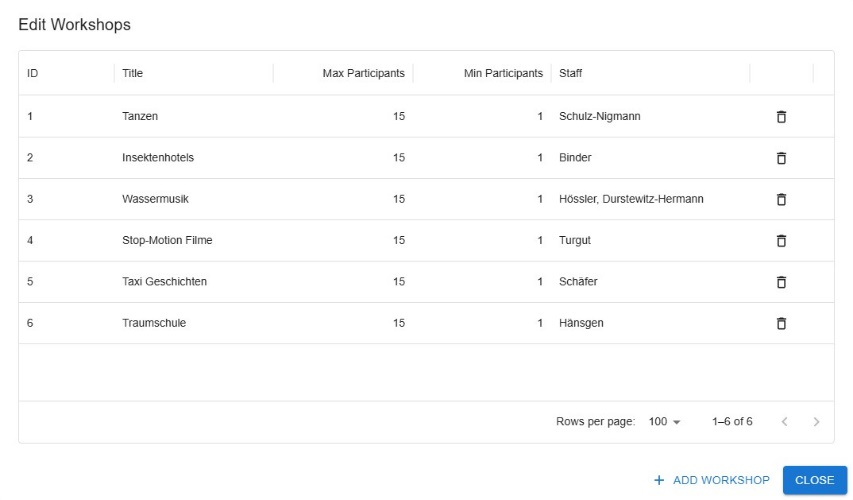
\includegraphics[width=3.88in]{image6.jpeg}
\end{center}

\subsection*{Eigenschaften bearbeiten}

\begin{itemize}
  \item Name
  \item Maximale Teilnehmerzahl
  \item Minimale Teilnehmerzahl
  \item Veranstaltende Person (\textbf{staff})
  % NEU
  \item Ort bzw. Raum (\textbf{location})
  \item Aktionsspalte
\end{itemize}

\subsection*{Mülleimer-Button}

\begin{itemize}
  \item Löscht einen Workshop.
\end{itemize}

% GEÄNDERT
\textbf{Wichtig:} Die Namen der Workshops müssen sich unterscheiden. Es darf keinen Workshop mit demselben Namen geben
(Groß- und Kleinschreibung und Leerzeichen am Rand werden dabei nicht beachtet). Jeder Workshop braucht außerdem eine
maximale Teilnehmerzahl von mindestens~1; die minimale Teilnehmerzahl darf nicht größer als die maximale sein.
Andernfalls wird die Zuteilung mit einer Fehlermeldung abgebrochen.

\section{Zuteilung}\label{sec:zuteilung}

\begin{mitbild}{2.68}{image7.png}
  % GEÄNDERT
  Eine Zuteilung kann über den Menüpunkt \emph{Zuteilung} im Menü \emph{Zuteilungen} erstellt werden. Möchte man eine neue
  Zuteilung erstellen, wird der Menüpunkt erneut ausgewählt; die bisherige Zuteilung wird dabei ersetzt. Mit
  \emph{Zuweisung zurücksetzen} wird die aktuelle Zuteilung verworfen.

  Personen können händisch per Rechtsklick in der Tabelle zugewiesen werden (Abschnitt~\ref{sec:haendisch}).

  Tritt ein Fehler bei der Zuteilung auf, oder ist eine Person nicht zuteilbar, wird der Nutzer darauf hingewiesen
  (Abschnitt~\ref{sec:meldungen}).
\end{mitbild}

Möchte man eine Zuteilung exportieren gibt es die folgenden Möglichkeiten:

\textbf{HTML:} Erstellt eine \textbf{Zuteilung} als HTML-Datei.

\textbf{CSV}: Erstellt eine \textbf{Zuteilung} als CSV-Datei.

\textbf{DOCX}: Erstellt eine \textbf{Zuteilung} als bearbeitbares Word-Dokument.

% NEU
\textbf{Excel}: Erstellt eine \textbf{Zuteilung} als Excel-Datei (\texttt{.xlsx}) mit mehreren Blättern:
\begin{itemize}
  \item \emph{Übersicht}: Belegung jedes Workshops (bei mehreren Tagen je Tag) mit Betreuung, Ort, Teilnehmerzahl und
  einem Hinweis, wenn ein Workshop unter dem Minimum liegt, über dem Maximum oder leer ist.
  \item \emph{Nach Workshop}: die Teilnehmerlisten.
  \item \emph{Nach Teilnehmer}: für jede Person der zugeteilte Workshop (bei mehreren Tagen eine Spalte pro Tag) und welcher
  Wunsch erfüllt wurde. Hier stehen auch Personen, die \emph{nicht zugeteilt} wurden, und Personen aus der
  Teilnehmerliste, die \emph{keine Präferenzen abgegeben} haben.
  \item \emph{Statistik}: dieselben Zahlen wie die Auswertung im Hauptfenster, einschließlich des Seeds.
  \item \emph{Warnungen}: alle Meldungen der Zuteilung.
\end{itemize}
Die Angaben zu Teilnehmerzahl, Personal und Raum richten sich nach den Einstellungen zur Berichtserstellung.

% GEÄNDERT
\textbf{Wichtig}: Die Zuteilung basiert auf dem Namen. Namen werden ohne Beachtung von Groß- und Kleinschreibung und
überzähligen Leerzeichen verglichen. Geben zwei Personen den gleichen Vor- und Nachnamen an, wird nur die erste Abgabe
berücksichtigt und es erscheint eine Warnung.

Neben der Tabelle mit allen Präferenzen gibt es eine Ansicht, welche nach einer Zuteilung bereits anzeigt, wie voll welche
Workshops sind, und eine Auswertung der Zuteilung (Abschnitt~\ref{sec:auswertung}).

% NEU
\subsection{So arbeitet die Zuteilung}\label{sec:algorithmus}

Die Zuteilung arbeitet nach einem einfachen Verfahren:
\begin{enumerate}
  \item Alle Personen werden in zufälliger Reihenfolge durchgegangen.
  \item Jede Person bekommt ihren ersten Wunsch, der noch einen freien Platz hat.
  \item Erreicht ein Workshop die Mindestteilnehmerzahl nicht, wird er nicht durchgeführt. Seine Teilnehmenden werden auf
  ihre übrigen Wünsche verteilt, soweit dort noch Plätze frei sind.
  \item Wer in keinem seiner Wünsche einen Platz bekommt, bleibt \textbf{nicht zugeteilt}. Es wird niemand automatisch in
  einen Workshop gesteckt, den er sich nicht gewünscht hat. Diese Personen stehen in der Auswertung und können
  händisch zugewiesen werden (Abschnitt~\ref{sec:haendisch}).
\end{enumerate}
Weil die Reihenfolge zufällig ist, sieht jede neue Zuteilung etwas anders aus. Das Verfahren ist darauf ausgelegt,
möglichst vielen Personen ihre erste Wahl zu geben (Abschnitt~\ref{sec:durchlaeufe}).

\subsection{Mehrere Tage}\label{sec:mehrtage}

In den Einstellungen können bis zu sieben Tage eingestellt werden. Bei mehreren Tagen bekommt jede Person für jeden Tag
einen Workshop, und niemand besucht denselben Workshop zweimal. Jeder Workshop findet an jedem Tag statt, mit der
eingestellten maximalen und minimalen Teilnehmerzahl \emph{pro Tag}.
\begin{itemize}
  \item Es müssen mindestens so viele Workshops angelegt sein wie Tage, sonst erscheint eine Fehlermeldung.
  \item Haben die Teilnehmenden weniger Wünsche als Tage, können nicht alle Tage über Wünsche besetzt werden. Die übrigen
  Tage bleiben offen und müssen händisch zugewiesen werden. Darauf weist eine Warnung hin.
  \item In der Tabelle steht in einer grünen Zelle zusätzlich der Tag als kleine Zahl.
  \item Im rechten Bereich ist jeder Workshop ein ausklappbarer Block. Zugeklappt steht die Belegung als Bereich, z.\,B.
  \emph{2--3/8}: An den Tagen sind zwischen 2 und 3 von 8 Plätzen belegt. Aufgeklappt erscheint jeder Tag einzeln. Rot
  bedeutet überfüllt, Orange unter dem Minimum. Mit \emph{Alle ausklappen} bzw. \emph{Alle einklappen} werden alle
  Blöcke auf einmal geöffnet oder geschlossen.
  \item Ändert man die Anzahl der Tage in den Einstellungen, wird die bisherige Zuteilung verworfen.
\end{itemize}

\subsection{Durchläufe und Seed}\label{sec:durchlaeufe}

In den Einstellungen kann die Anzahl der \textbf{Durchläufe} (1 bis 200) festgelegt werden. Bei mehr als einem Durchlauf
wird die Zuteilung mehrfach mit anderen Zufallswerten durchgeführt und der Durchlauf mit den \textbf{meisten ersten
Wahlen} übernommen (bei Gleichstand der mit weniger nicht zugeteilten Personen). Mehr Durchläufe bringen meist mehr erste
Wahlen, können aber dazu führen, dass etwas mehr Personen offen bleiben. Auch 200 Durchläufe dauern nur Bruchteile einer
Sekunde.

Die Auswertung zeigt dann \emph{Bester von N Durchläufen} und den \textbf{Seed}. Der Seed ist die Startzahl des Zufalls:
Dieselben Daten mit demselben Seed ergeben dieselbe Zuteilung.

\subsection{Auswertung}\label{sec:auswertung}

\begin{mitbild}{2.30}{image8.png}
  Rechts neben der Tabelle steht oben die \textbf{Auswertung} der aktuellen Zuteilung. Ein Klick auf die Kopfzeile klappt sie
  auf oder zu; der Zustand wird gemerkt. Zugeklappt zeigt sie eine Kurzfassung, z.\,B. \emph{56\,\% 1.~Wahl · 3 offen}.
  \begin{itemize}
    \item \emph{Zuteilungen} (bei mehreren Tagen \emph{Tageszuteilungen}): wie viele Zuteilungen es gibt.
    \item \emph{1.~Wahl}, \emph{2.~Wahl} usw.: wie vielen Zuteilungen der jeweilige Wunsch entspricht, mit Prozentwert.
    \item \emph{Ohne Wunsch zugeteilt}: Zuteilungen, die nicht aus den Wünschen stammen, also händisch vorgenommene.
    \item \emph{Nicht zugeteilt}: Personen ohne Platz. \emph{Namen anzeigen} listet sie auf, bei mehreren Tagen mit dem
    jeweiligen Tag.
    \item \emph{Freie Plätze}: freie von allen Plätzen.
    \item \emph{unter Minimum / nicht durchgeführt}: Workshops (bei mehreren Tagen je Tag), die die Mindestzahl nicht
    erreichen.
    \item \emph{Bester von N Durchläufen} und \emph{Seed} (Abschnitt~\ref{sec:durchlaeufe}).
  \end{itemize}
  Die Auswertung rechnet nach jeder händischen Änderung neu. Darunter steht die Belegung jedes Workshops
  (\emph{Belegung/Maximum}, rot bei Überfüllung).
\end{mitbild}

\subsection{Händisch zuweisen}\label{sec:haendisch}

\begin{mitbild}{2.99}{image22.png}
  Ein \textbf{Rechtsklick} auf einen Namen oder einen Wunsch in der Tabelle öffnet das Menü zum Zuweisen:
  \begin{itemize}
    \item \emph{„Workshop“ zuweisen}: weist den Workshop der angeklickten Wahl zu (nur beim Klick auf einen Wunsch).
    \item \emph{Anderen Workshop zuweisen}: Liste aller Workshops mit ihrer aktuellen Belegung. Hier lassen sich auch
    Workshops zuweisen, die nicht gewünscht wurden, z.\,B. für Personen, die nicht zugeteilt werden konnten.
    \item \emph{Zuweisung aufheben}: gibt den Platz der Person wieder frei.
  \end{itemize}
\end{mitbild}

\begin{mitbild}{3.53}{image23.png}
  Bei \textbf{mehreren Tagen} fragt das Menü nach dem Tag (\emph{Tag 1}, \emph{Tag 2}, \dots), wie im Bild oben. Bei
  \emph{Anderen Workshop zuweisen} öffnet sich zuerst die Liste der Workshops und danach die Auswahl des Tages (Bild
  rechts). Ein Häkchen zeigt, dass die Person den Workshop an diesem Tag schon hat; steht dort \emph{ersetzt: \dots},
  wird die bisherige Zuweisung dieses Tages überschrieben. Wird ein Workshop, den die Person schon an einem anderen Tag
  hat, für einen neuen Tag gewählt, wird er verschoben, denn niemand besucht denselben Workshop zweimal. So können alle
  Tage einzeln zugewiesen werden.
\end{mitbild}

\begin{itemize}
  \item Das Zuweisen funktioniert auch \emph{ohne} vorherige Zuteilung: Dann entsteht eine leere Zuteilung nach den
  Einstellungen (Anzahl Tage), in die man von Hand zuweisen kann.
  \item Die Plätze werden nicht geprüft. Weist man mehr Personen zu als Plätze da sind, wird der Workshop rot angezeigt,
  und man entscheidet selbst.
  \item Händische Zuweisungen gehen verloren, wenn eine neue Zuteilung erstellt wird.
\end{itemize}

\subsection{Meldungen bei der Zuteilung}\label{sec:meldungen}

Nach der Zuteilung erscheint bei Auffälligkeiten ein Fenster mit den Warnungen (bei mehr als zwölf werden die ersten
gezeigt). Häufige Meldungen:
\begin{itemize}
  \item \emph{Der Workshop-Titel \dots{} kommt mehrfach vor}: Zwei Workshops heißen gleich. Einen davon umbenennen.
  \item \emph{Der Workshop \dots{} hat keine gültige maximale Teilnehmerzahl}: Die maximale Teilnehmerzahl fehlt oder ist
  kleiner als~1. Es wird keine Zuteilung erstellt, bis dies behoben ist.
  \item \emph{Bei N Tagen werden mindestens N verschiedene Workshops benötigt}: Mehr Tage als Workshops.
  \item \emph{Der Wunsch \dots{} passt zu keinem Workshop}: In einer Präferenz steht ein Name, den es als Workshop nicht
  gibt (Tippfehler oder Workshop umbenannt). Der Wunsch wird ignoriert.
  \item \emph{\dots{} hat in keinem Wunsch-Workshop einen Platz bekommen und ist nicht zugeteilt}: Die Person bleibt offen
  und kann von Hand zugewiesen werden.
  \item \emph{Der Workshop \dots{} hat das Minimum \dots{} nicht erreicht und wird nicht durchgeführt}.
  \item \emph{Es gibt nur X Plätze für Y Teilnehmer}: Insgesamt sind zu wenige Plätze angelegt.
  \item \emph{\dots{} hat mehrfach abgegeben}: Es wird nur die erste Abgabe berücksichtigt.
\end{itemize}

\section{Teilnehmer}\label{sec:teilnehmer}

\subsection*{Import}

\begin{mitbild}{1.76}{image9.jpeg}
  \begin{itemize}
    % GEÄNDERT
    \item Importiert eine Liste von Teilnehmenden aus einer Excel-Datei (\texttt{.xlsx}), einer CSV-Datei oder einer
    JSON-Datei. Die Spalten können im Import-Dialog frei zugeordnet werden (Abschnitt~\ref{sec:importdialog}).
  \end{itemize}

  \textbf{JSON-Format:} Array von Objekten mit \texttt{Vorname}, \texttt{Name}, \texttt{Kurs} (Kurs ist optional).

  % GEÄNDERT
  \textbf{Excel- und CSV-Format:} Eine Zeile pro Person mit den Spalten \texttt{Nachname}, \texttt{Vorname} und optional
  \texttt{Kurs}. Bei CSV-Dateien kann als Trennzeichen \textbf{\texttt{,}} oder \textbf{\texttt{;}} (oder ein Tabulator)
  verwendet werden. Die Spaltenüberschriften werden automatisch erkannt, auch in anderer Reihenfolge. Unterstützte
  Überschriften sind zum Beispiel:
  \begin{itemize}
    \item \texttt{Nachname}, \texttt{Familienname}, \texttt{Lastname}, \texttt{Name}
    \item \texttt{Vorname}, \texttt{Firstname}
    \item \texttt{Kurs}, \texttt{Klasse}, \texttt{Gruppe}
  \end{itemize}
\end{mitbild}
Fehlt die Überschriftenzeile oder wird eine Überschrift nicht erkannt, ordnet man die Spalten im Import-Dialog selbst zu.
Ohne Überschrift wird als Reihenfolge \texttt{Nachname}, \texttt{Vorname} angenommen; der Dialog kennzeichnet das als
\emph{geraten – bitte prüfen}.

Zusätzlich gibt es \textbf{Teilnehmer exportieren} im Menü \emph{Datei}: Die Liste wird als Excel-Datei oder im
\texttt{.json}-Format gespeichert (Abschnitt~\ref{sec:exportdialog}).

\textbf{Beispiel-Datei} (\texttt{participants.json}):
\begin{Verbatim}[frame=single,fontsize=\small]
[
  {"Vorname": "Max", "Name": "Mustermann"},
  {"Vorname": "Erika", "Name": "Musterfrau"}
]
\end{Verbatim}

\textbf{Beispiel-Datei} (\texttt{participants.csv}):
\begin{Verbatim}[frame=single,fontsize=\small]
Nachname; Vorname
Mustermann; Max
Musterfrau; Erika
\end{Verbatim}

% NEU
\section{Import-Dialog (Excel, CSV, JSON)}\label{sec:importdialog}

Präferenzen, Workshops und Teilnehmer werden über denselben Dialog importiert. Er öffnet sich über das Menü \emph{Datei}
\pfeil{} \emph{Präferenzen importieren}, \emph{Workshops importieren} oder \emph{Teilnehmer importieren} und zeigt
immer nur die gewählte Art. Erlaubt sind Excel-Dateien (\texttt{.xlsx}), CSV-Dateien (\texttt{.csv}, Trennzeichen
\texttt{;}, \texttt{,} oder Tabulator) und JSON-Dateien (\texttt{.json}). Alte Excel-Dateien (\texttt{.xls}) müssen vorher in
Excel über \emph{Speichern unter} als \texttt{.xlsx} gespeichert werden. Die Datei darf höchstens 10~MB groß sein, es
werden bis zu 5000 Zeilen gelesen.
\bild{5.60}{image24.png}

\subsection*{Ablauf}

\begin{enumerate}
  \item \textbf{Datei wählen}: auf \emph{Datei auswählen} klicken oder die Datei in das Fenster ziehen.
  \item Wer keine passende Datei hat, klickt auf \textbf{Excel-Vorlage herunterladen}: Die Vorlage enthält die richtigen
  Überschriften, zwei Beispielzeilen und ein Blatt mit Hinweisen.
  \item Enthält die Datei \textbf{mehrere Blätter}, wird das passende vorgewählt; es lässt sich oben ändern. Mit dem
  Häkchen \emph{Erste Zeile enthält Spaltenüberschriften} wird festgelegt, ob die erste Zeile Überschriften sind.
  \item \textbf{Spalten prüfen}: Über jeder Spalte steht ein Auswahlfeld. Der Dialog erkennt die Spalten selbst und füllt es
  vor (auch bei anderen Überschriften, z.\,B. \emph{Plätze} für die maximale Teilnehmerzahl oder \emph{Erstwahl} für die
  1.~Wahl). Orange mit dem Hinweis \emph{geraten – bitte prüfen} sind Zuordnungen, die nur nach der Position der Spalte
  vorgeschlagen wurden. Pflichtfelder sind mit \emph{*} gekennzeichnet. Spalten, die nicht gebraucht werden, bleiben
  auf \emph{– nicht verwenden –}.
  \item \textbf{Prüfung lesen}: Unter der Vorschau steht, wie viele Zeilen importiert werden. Zeilen mit Fehlern werden
  übersprungen; sie sind mit der \textbf{Zeilennummer wie in Excel} aufgeführt.
  \item Wählen, ob die vorhandenen Einträge \textbf{ersetzt} oder die neuen \textbf{angehängt} werden (beim Anhängen werden
  Doppelte übersprungen).
  \item Auf \emph{N Einträge importieren} klicken.
\end{enumerate}
\bild{5.60}{image25.png}

Das Speichern der importierten Einträge erfolgt ganz oder gar nicht: Tritt dabei ein Fehler auf, bleiben die vorhandenen
Daten unverändert. Eine sinnvolle Reihenfolge ist: erst die Workshops, dann die Teilnehmer, dann die Präferenzen, weil die Präferenzen
gegen die Workshops geprüft werden.

\subsection*{Erwartete Spalten}

\begin{longtable}{@{}p{0.2\linewidth}p{0.74\linewidth}@{}}
  \toprule
  \textbf{Art} & \textbf{Spalten} (\emph{*} = Pflicht) \\
  \midrule
  \endhead
  Teilnehmer & Vorname*, Nachname*, Kurs \\
  Workshops & Titel*, Min.~Teilnehmer, Max.~Teilnehmer*, Betreuung, Ort \\
  Präferenzen & Name* (Vor- und Nachname in einer Spalte), 1.~Wahl*, 2.~Wahl, \dots, bis 7.~Wahl \\
  \bottomrule
\end{longtable}

\subsection*{Was geprüft wird}

\begin{itemize}
  \item \textbf{Workshops}: Der Titel darf nicht fehlen oder doppelt vorkommen. Die maximale Teilnehmerzahl muss eine Zahl
  von mindestens~1 sein. Ist das Minimum größer als das Maximum, wird die Zeile übersprungen mit dem Hinweis, dass die
  Spalten vertauscht sein könnten.
  \item \textbf{Präferenzen}: Wünsche werden mit den vorhandenen Workshops verglichen. Eine andere Groß- und
  Kleinschreibung oder überflüssige Leerzeichen werden korrigiert. Wünsche, zu denen es keinen Workshop gibt, werden
  gemeldet und mit aufgeführt; bei der Zuteilung werden sie ignoriert. Weiter wird gemeldet, wenn jemand denselben
  Workshop mehrfach gewählt hat oder ein Name doppelt vorkommt, und wie viele Namen zur Teilnehmerliste passen. Passt
  mehr als die Hälfte der Wünsche zu keinem Workshop, fragt der Dialog, ob die richtigen Spalten zugeordnet wurden.
  \item \textbf{Teilnehmer}: Fehlt Vor- oder Nachname oder kommt eine Person doppelt vor, wird die Zeile übersprungen.
  Wenn schon Präferenzen vorhanden sind, vergleicht der Dialog die Namen mit ihnen. Passen sie nur mit vertauschtem Vor-
  und Nachnamen, erscheint ein Hinweis mit dem Knopf \emph{Tauschen}.
\end{itemize}

\section{Export-Dialog (Excel, JSON)}\label{sec:exportdialog}

\begin{mitbild}{2.04}{image26.jpg}
  Das Menü \emph{Datei} enthält zu jeder Art einen Export:
  \begin{itemize}
    \item \textbf{Präferenzen exportieren}, \textbf{Workshops exportieren}, \textbf{Teilnehmer exportieren}: Der Dialog zeigt
    die Anzahl der Einträge und lässt wählen zwischen \emph{Excel (.xlsx)} und \emph{JSON (Sicherung)}. Die Dateien heißen
    z.\,B. \texttt{Praeferenzen\_2026-10-13.xlsx} bzw.\ \texttt{submissions.json}, \texttt{workshops.json} und
    \texttt{participants.json}.
    \item \textbf{Alles als Excel exportieren\dots}: Alles Angehakte (Präferenzen, Workshops, Teilnehmer und, wenn vorhanden,
    die Zuteilung) kommt in \emph{eine} Excel-Datei, jeweils auf einem eigenen Blatt
    (\texttt{Semera-Workshops\_<Datum>.xlsx}).
  \end{itemize}
  Alle Dateien lassen sich später mit dem Import-Dialog wieder einlesen. Das ist auch eine gute \textbf{Sicherung} vor einem
  Update.

  Die Excel-Blätter für Präferenzen, Workshops und Teilnehmer haben dieselben Überschriften wie die Vorlage des
  Import-Dialogs: Teilnehmer \emph{Vorname, Nachname, Kurs}; Workshops \emph{Titel, Min.\ Teilnehmer, Max.\ Teilnehmer,
  Betreuung, Ort}; Präferenzen \emph{Name, 1.~Wahl, 2.~Wahl, \dots}. Die Blätter der Zuteilung sind in Abschnitt~\ref{sec:zuteilung}
  beschrieben.
\end{mitbild}

\section{Ansicht}\label{sec:ansicht}

\begin{mitbild}{2.60}{image10.jpeg}
  \textbf{Ansicht aktualisieren:} Aktualisiert die Ansicht.

  \textbf{Abgabe-Formular öffnen:} Öffnet das Abgabe-Formular im Standard-Browser.
\end{mitbild}

\begin{mitbild}{2.91}{image11.png}
  \textbf{Fehlende Teilnehmer:} Zeigt eine Liste der Personen ohne Präferenzen.
\end{mitbild}

\begin{mitbild}{4.14}{image12.jpeg}
  \textbf{QR Code:}\label{sec:qr} Öffnet einen Dialog mit einem QR-Code zum einfachen Zugriff.

  Falls hierbei ein Fehler auftritt, sollte dieser angezeigt werden. ACHTUNG: Trennt man die Verbindung des Computers zum Netzwerk, kann sich die IP-Adresse des Computers ändern, das bedeutet, dass ein älterer QR-Code für „Android/ Andere“ nicht mehr funktioniert. Eine feste Adresse für den Rechner schafft Abhilfe (Abschnitt~\ref{sec:netzwerk}).
\end{mitbild}

% NEU
Im Dialog gibt es zwei QR-Codes:
\begin{itemize}
  \item \textbf{Android / Andere} enthält die IP-Adresse des Rechners (und den Port, wenn er nicht 80 ist).
  \item \textbf{iOS} enthält den Namen \texttt{semera.local}. Er funktioniert auf iPhones, solange der Router die
  Namensauflösung im WLAN (mDNS/Bonjour) nicht blockiert, und ändert sich nicht, wenn sich die IP-Adresse ändert.
  Funktioniert er nicht, kann man auch auf dem iPhone den Android-Code verwenden.
\end{itemize}
Oben im Dialog steht das Auswahlfeld \textbf{Verfügbare Netzwerkadapter}. Ein Rechner hat oft mehrere
Netzwerkadapter (WLAN, LAN, VirtualBox, VPN \dots), und nur einer davon ist für die Handys erreichbar.
\begin{itemize}
  \item \emph{Automatisch} wählt den besten echten WLAN- oder LAN-Adapter. Virtuelle Adapter (VirtualBox, VMware,
  WSL, Docker), VPN-Netze und Adapter ohne gültige Adresse werden erkannt und nicht gewählt. Das Netz eines
  Windows-Hotspots (\texttt{192.168.137.x}) wird ausdrücklich zugelassen.
  \item Die Liste zeigt alle Adapter mit Adresse und einer Kennzeichnung (\emph{virtuell}, \emph{VPN}, \dots). Eine eigene
  Auswahl bleibt gespeichert. Wählt man einen ungeeigneten Adapter, erscheint eine Warnung.
  \item Nach einem Wechsel des Netzwerks oder wenn sich die Adresse ändert, meldet sich der Rechner nach etwa 15 Sekunden
  im Netz mit der neuen Adresse an (gilt für \texttt{semera.local}). Der QR-Code für Android muss dann neu angezeigt
  werden.
\end{itemize}

\section{Einstellungen}\label{sec:einstellungen}

\begin{mitbild}{1.77}{image13.jpeg}
  Die Einstellungen werden über das Menü \emph{Datei} \pfeil{} \emph{Einstellungen\dots} geöffnet.

  \medskip\textbf{Allgemein}\par\nopagebreak

  \begin{itemize}
    \item Einstellung zum Warnen vor dem Löschen einzelner Einträge.
  \end{itemize}

  \medskip\textbf{Workshop Einstellungen}\par\nopagebreak

  \begin{itemize}
    % GEÄNDERT
    \item Auswahl der \textbf{Tagesanzahl} (1 bis 7) und der \textbf{Anzahl der Wahlen} (1 bis 7). Die Teilnehmeransicht zeigt
    entsprechend viele Felder, und die Tabelle entsprechend viele Wahl-Spalten.
    % NEU
    \item \textbf{Durchläufe} (1 bis 200): Wie oft die Zuteilung wiederholt wird; der Durchlauf mit den meisten ersten Wahlen
    wird übernommen (Abschnitt~\ref{sec:durchlaeufe}). Standard ist 1.
  \end{itemize}
  Eine Änderung der Tagesanzahl verwirft die aktuelle Zuteilung. Es müssen mindestens so viele Workshops angelegt sein
  wie Tage.
\end{mitbild}

\begin{mitbild}{3.66}{image14.png}
  \textbf{Berichtserstellung} Einstellung, ob bestimmte Informationen im erstellten Bericht sichtbar sein sollen.

  \begin{itemize}
    \item Teilnehmerzahl/ maximale Teilnehmer anzeigen (zB 8/10)
    \item Personal anzeigen (Wer für den Workshop zuständig ist)
    \item Raum anzeigen (Wo der Workshop stattfindet)
  \end{itemize}

  \medskip\textbf{Netzwerk}\par\nopagebreak

  \begin{itemize}
    \item Bonjour/ mDNS aktivieren (sollte immer an bleiben, nur deaktivieren, wenn es Probleme mit Bonjour oder den .local Adressen gibt).
    % NEU
    Damit ist der Rechner im WLAN auch unter dem Namen \texttt{semera.local} erreichbar, den der QR-Code für iPhones
    verwendet.
    \item Port anpassen (Standard 80, sollte immer 80 bleiben, es sei denn der Port wird durch eine andere App blockiert).
    % NEU
    Wird der Port geändert, ändern sich auch die QR-Codes, bereits gedruckte Codes sind dann ungültig.
  \end{itemize}
\end{mitbild}

\section{Hilfe}

\begin{mitbild}{3.30}{image15.jpeg}
  \textbf{Handbuch (PDF):} Öffnet dieses Handbuch.

  \textbf{Über:} Informationen zu dieser Software.
\end{mitbild}

\section{Statusanzeige}

\begin{mitbild}{2.08}{image16.jpeg}
  Unten links wird angezeigt, wie viele Personen bereits eine \textbf{passende Zuteilung} haben.
\end{mitbild}

% NEU
Unten rechts löscht der Knopf \textbf{Alle löschen} nach einer Rückfrage alle Präferenzen. Das lässt sich nicht
rückgängig machen, deshalb vorher mit \emph{Datei} \pfeil{} \emph{Alles als Excel exportieren\dots} eine Sicherung anlegen.

\section{Teilnehmeransicht}\label{sec:teilnehmeransicht}

\begin{mitbild}{2.80}{image17.jpeg}
  Hier geben die Teilnehmenden ihre Präferenzen ab. Die Teilnehmeransicht kann über den QR-Code oder die URL unterhalb des QR-Codes aufgerufen werden.

  \medskip\textbf{Name eintragen}\par\nopagebreak

  \begin{itemize}
    \item Format: \texttt{Vorname Nachname}
    \bild{2.84}{image18.jpeg}
  \end{itemize}

  \medskip\textbf{Wünsche auswählen}\par\nopagebreak

  \begin{itemize}
    % GEÄNDERT
    \item Alle Wünsche auswählen, so viele wie in den Einstellungen festgelegt sind (bis zu sieben). Jeder Workshop kann
    nur einmal gewählt werden, und alle Wünsche müssen ausgefüllt sein.
  \end{itemize}
\end{mitbild}

\subsection*{Abschicken}

\begin{mitbild}{2.07}{image19.jpeg}
  \begin{itemize}
    \item Button \textbf{Auswahl abschicken} klicken.
    \item Daten werden gespeichert und eine \textbf{Bestätigungsmeldung} angezeigt.
  \end{itemize}
\end{mitbild}

% NEU
\subsection*{Bei schlechter Verbindung}

\begin{itemize}
  \item Die Seite ist klein (etwa 90~KB) und lädt auch bei vielen gleichzeitigen Handys schnell. Beim Laden wird bei
  Problemen automatisch mehrfach versucht; hilft das nicht, erscheint \emph{Erneut versuchen}, ohne die Seite neu zu
  laden.
  \item Kommt das Handy aus dem Ruhezustand und das WLAN ist noch nicht wieder da, bleibt das ausgefüllte Formular
  stehen.
  \item Während des Sendens ist der Knopf gesperrt (\emph{Wird gesendet \dots}). Nach etwa 12 Sekunden ohne Antwort erscheint
  \emph{Keine Verbindung zum Server}. Die Auswahl bleibt erhalten; nach Prüfung des WLANs einfach noch einmal auf
  \emph{Auswahl abschicken} tippen.
  \item \textbf{Doppelt senden schadet nicht.} Hat der Rechner die Abgabe schon erhalten, die Antwort ist aber verloren
  gegangen, wird dieselbe Abgabe beim zweiten Mal als bereits gespeichert erkannt. Die Meldung \emph{Du hast deine Wünsche
  bereits eingereicht} erscheint nur, wenn unter demselben Namen \emph{andere} Wünsche abgegeben werden.
\end{itemize}

\subsection*{Zugriff nur für die Abgabe}

Handys können nur Wünsche abgeben und die Liste der Workshops sehen. Verwaltung, Import, Löschen und Zuteilen sind aus
Sicherheitsgründen nur an dem Rechner möglich, auf dem das Programm läuft. Die Verwaltungsseite (\texttt{/admin}) ist vom
Handy aus nicht erreichbar.

% NEU
\section{Netzwerk und Router}\label{sec:netzwerk}

Die Handys erreichen das Programm über das WLAN. Es wird \textbf{kein Internet} gebraucht, Handys und Rechner müssen nur
im selben Netz sein. Am zuverlässigsten ist ein \textbf{eigener kleiner Router} (oder Access Point im Router-Modus) nur für
den Workshop: Dort stimmen die Einstellungen, und der Rechner bekommt immer dieselbe Adresse, sodass gedruckte
QR-Codes immer gültig bleiben.

\subsection{Einstellungen am Router}

Die Menüs unterscheiden sich je nach Hersteller, Modell und Firmware. Gesucht werden diese Funktionen:
\begin{enumerate}
  \item \textbf{Gleiches Netz}: Handys und Rechner im selben WLAN. Ein \emph{Gastnetz} ist meist ungeeignet, denn es ist
  vom restlichen Netz getrennt (bei der FRITZ!Box vollständig).
  \item \textbf{Geräte-Trennung ausschalten}: Sie heißt \emph{AP-Isolation}, \emph{Client Isolation}, \emph{Wireless
  Isolation}, \emph{Geräte dürfen untereinander kommunizieren} o.\,Ä. Ist sie an, sehen sich Handy und Rechner nicht. Bei
  der FRITZ!Box: \emph{WLAN} \pfeil{} \emph{Sicherheit}, \emph{Aktive WLAN-Geräte dürfen untereinander kommunizieren}.
  \item \textbf{DHCP einschalten}: Der Router muss Adressen verteilen (meist Werkseinstellung).
  \item \textbf{Kein Internet nötig}: Die Handys melden \emph{Verbunden, kein Internet}. Das ist normal. Die Verbindung
  behalten und \textbf{mobile Daten ausschalten}, sonst schicken manche Handys die Anfragen am WLAN vorbei.
  \item \textbf{Keine Portfreigabe}, keine DMZ, keine Freigabe ins Internet. Alles bleibt im lokalen Netz.
  \item \textbf{mDNS/Bonjour (Multicast) nicht blockieren}: Der QR-Code für iPhones (\texttt{semera.local}) braucht das.
  Funktioniert es nicht, den Android-Code (IP-Adresse) verwenden.
  \item \textbf{Viele Geräte}: Ab etwa 15 bis 30 Handys lieber einen eigenen Router verwenden. Der Windows-Hotspot ist
  nach Angaben aus der Community auf 8 Geräte begrenzt (von Microsoft nicht bestätigt).
  \item \textbf{Schul-, Hotel- und Gastnetze} haben meist Geräte-Trennung und Anmeldeseiten. Dort funktioniert es in der
  Regel nicht; einen eigenen Router mitbringen.
\end{enumerate}

\subsection{Feste Adresse für den Rechner}\label{sec:feste-ip}

Ändert sich die Adresse des Rechners, ändert sich auch der QR-Code für Android. Mit einer festen Adresse kann man die
QR-Codes einmal drucken. Es gibt zwei Wege.

\subsubsection*{Weg 1 (empfohlen): DHCP-Reservierung im Router}

Der Rechner bleibt auf \emph{automatisch}, und der Router gibt ihm immer dieselbe Adresse.
\begin{enumerate}
  \item Die \textbf{MAC-Adresse} des Rechners herausfinden. Unter Windows: Eingabeaufforderung, \texttt{ipconfig /all}, Zeile
  \emph{Physische Adresse} des WLAN- oder LAN-Adapters.
  \item Im Router die Reservierung anlegen. Gesucht wird \emph{DHCP-Reservierung}, \emph{Address Reservation},
  \emph{Static DHCP / Static Lease} oder \emph{IP Binding / Manual Assignment}. Bei der FRITZ!Box: das Gerät bearbeiten und
  \emph{Diesem Netzwerkgerät immer die gleiche IPv4-Adresse zuweisen} anhaken.
  \item Den Rechner neu mit dem WLAN verbinden, damit er die Adresse übernimmt.
\end{enumerate}
\textbf{Fallstrick Zufalls-Adresse:} Wechselt die MAC-Adresse des Rechners, greift die Reservierung nicht mehr. Unter
Windows heißt die Einstellung \emph{Zufällige Hardware-Adressen verwenden} (in den Eigenschaften des WLANs), auf dem Mac
\emph{Private WLAN-Adresse}. Für das Workshop-WLAN ausschalten (beim Mac ist auch \emph{Fest} in Ordnung, nicht aber
\emph{Rotierend}).

\subsubsection*{Weg 2: feste Adresse direkt am Rechner}

Wenn der Router keine Reservierung kann (z.\,B. einige ältere Speedport-Modelle), stellt man die Adresse am Rechner ein. Unter
Windows meist über \emph{Einstellungen} \pfeil{} \emph{Netzwerk \& Internet} \pfeil{} \emph{WLAN} bzw.\ \emph{Ethernet} \pfeil{}
\emph{IP-Zuweisung} \pfeil{} \emph{Bearbeiten} \pfeil{} \emph{Manuell} (je nach Windows-Version leicht anders). Einzutragen sind:
\begin{itemize}
  \item eine Adresse im selben Netz, aber \textbf{außerhalb} des DHCP-Bereichs des Routers,
  \item die Subnetzmaske, meist \texttt{255.255.255.0},
  \item als Gateway und DNS-Server die Adresse des Routers.
\end{itemize}
In einem anderen Netz muss man wieder auf \emph{Automatisch (DHCP)} zurückstellen, sonst hat der Rechner dort keine
Verbindung.

\subsubsection*{Anleitungen der Hersteller}

Die Seiten beschreiben die Reservierung bzw.\ die Geräte-Trennung beim jeweiligen Hersteller (Stand der Recherche,
Menüs können sich ändern):
\begin{itemize}
  \item AVM FRITZ!Box, feste Adresse:\\
  \url{https://avm.de/service/wissensdatenbank/dok/FRITZ-Box-7170/201_Netzwerkgerat-immer-die-gleiche-IP-Adresse-von-FRITZ-Box-zuweisen-lassen/}
  \item AVM FRITZ!Box, Geräte untereinander:\\
  \url{https://avm.de/service/wissensdatenbank/dok/FRITZ-Box-4060/549_Kein-Zugriff-auf-andere-Gerate-im-FRITZ-Heimnetz-moglich/}
  \item AVM FRITZ!Box, Gastzugang:\\
  \url{https://ch.avm.de/service/wissensdatenbank/dok/FRITZ-Box-7583/294_WLAN-Gastzugang-in-FRITZ-Box-einrichten/}
  \item NETGEAR:\\
  \url{https://kb.netgear.com/25722/How-do-I-reserve-an-IP-address-on-my-NETGEAR-router}
  \item ASUS (die Adresse muss im DHCP-Bereich liegen):\\
  \url{https://www.asus.com/support/faq/1000906/}
  \item TP-Link, Address Reservation (Beispielmodell, das Menü weicht je nach Modell ab):\\
  \url{https://www.tp-link.com/de/support/faq/1657/}
  \item TP-Link, AP Isolation (Beispiel für Pharos/CPE-Geräte, bei Heimroutern kann die Einstellung anders heißen):\\
  \url{https://www.tp-link.com/de/support/faq/2089/}
  \item Telekom Speedport (Beitrag der Community, keine offizielle Anleitung; neuere Modelle wie der Smart~4 haben
  \emph{immer dieselbe IPv4-Adresse}, ältere nur Weg~2):\\
  \url{https://telekomhilft.telekom.de/conversations/festnetz-internet/speedport-smart-3-zuordnung-fester-ip-adressen/6688a3764ae73561dac3ee04}
\end{itemize}

\subsection{Windows-Hotspot statt Router}

Der Windows-Hotspot gibt dem Rechner meist fest die Adresse \texttt{192.168.137.1}. Das ist ohne Router stabil, aber auf
wenige Geräte begrenzt (siehe oben) und nur geeignet, wenn die WLAN-Karte das unterstützt.

\subsection{QR-Codes drucken}

\begin{itemize}
  \item Der \textbf{iPhone-Code} (\texttt{semera.local}) enthält keine IP-Adresse und bleibt gültig, solange der Router
  mDNS zulässt.
  \item Der \textbf{Android-Code} enthält die IP-Adresse \emph{und den Port}, wenn er nicht 80 ist. Er gilt nur, solange
  beides gleich bleibt. Wer ihn vorab drucken will, braucht eine feste Adresse (Abschnitt~\ref{sec:feste-ip}).
  \item Reihenfolge: erst Router und feste Adresse einrichten, dann im QR-Dialog das richtige Netzwerk wählen und prüfen,
  dann drucken.
  \item \textbf{Vor dem Termin testen}: mit einem Android-Handy und einem iPhone scannen, mobile Daten aus.
  \item Praktisch ist ein zweiter QR-Code mit dem WLAN-Namen und -Passwort daneben, den die Handy-Kamera ebenfalls
  liest.
  \item Ohne feste Adresse die QR-Codes erst am Termin aus dem Dialog zeigen (Beamer oder Bildschirm), statt sie vorab zu
  drucken.
\end{itemize}

\section{Probleme und Lösungen}\label{sec:probleme}

\textbf{Problem:} Teilnehmer kann die Seite nicht am Handy öffnen.

\textbf{Lösung:}\par\nopagebreak
\begin{itemize}
  \item Handy eines anderen Teilnehmers nutzen \textbf{oder}
  \item Wünsche direkt am Laptop eintragen, auf dem das Programm läuft.
\end{itemize}

% NEU
\textbf{Problem:} Die Seite lässt sich am Handy nicht öffnen oder lädt nicht.

\textbf{Lösung:}\par\nopagebreak
\begin{itemize}
  \item Sind Handy und Rechner im \textbf{selben WLAN}, nicht im Gastnetz (Abschnitt~\ref{sec:netzwerk})?
  \item Ist im Router die \textbf{Geräte-Trennung} (AP-/Client-Isolation) ausgeschaltet?
  \item Zeigt der QR-Dialog das \textbf{richtige Netzwerk}? Bei mehreren Adaptern im Auswahlfeld das WLAN bzw.\ LAN wählen
  (kein VirtualBox-, VPN- oder WSL-Adapter).
  \item \textbf{Mobile Daten am Handy ausschalten} und die Meldung \emph{Verbunden, kein Internet} bestätigen.
  \item Die \textbf{Firewall} des Rechners muss das Programm im privaten Netz zulassen. Beim ersten Start fragt Windows
  danach; dann \emph{Zugriff zulassen} wählen. Das WLAN darf nicht als \emph{öffentliches Netzwerk} eingestuft sein.
  \item Ist der \textbf{Port} (Standard 80) von einem anderen Programm belegt? Dann in den Einstellungen einen anderen Port
  wählen (die QR-Codes ändern sich).
\end{itemize}

\textbf{Problem:} Der QR-Code für iPhones (\texttt{semera.local}) funktioniert nicht.

\textbf{Lösung:} Den Android-Code (IP-Adresse) verwenden. Prüfen, ob in den Einstellungen \emph{Bonjour/mDNS aktivieren}
eingeschaltet ist und ob der Router mDNS durchlässt.

\textbf{Problem:} Der QR-Code für Android zeigt eine falsche oder veraltete Adresse.

\textbf{Lösung:} Im QR-Dialog das richtige Netzwerk wählen. Hat sich die Adresse des Rechners geändert, den Dialog neu
öffnen und den neuen Code zeigen. Für gedruckte Codes eine feste Adresse einrichten (Abschnitt~\ref{sec:feste-ip}).

\textbf{Problem:} Eine Person ist nach der Zuteilung \emph{nicht zugeteilt}.

\textbf{Lösung:} In keinem ihrer Wünsche war noch ein Platz frei. In der Auswertung auf \emph{Namen anzeigen} klicken
und die Person per Rechtsklick händisch zuweisen (Abschnitt~\ref{sec:haendisch}). Alternativ mehr Plätze schaffen und die
Zuteilung wiederholen, oder die Anzahl der Durchläufe erhöhen.

\textbf{Problem:} Beim Import erscheint eine Fehlermeldung oder Zeilen werden übersprungen.

\textbf{Lösung:} Die Zeilennummer im Hinweis entspricht der Zeile in Excel. Häufige Ursachen: Pflichtfeld leer, maximale
Teilnehmerzahl keine Zahl, doppelter Name oder Titel, Spalten falsch zugeordnet. Ältere \texttt{.xls}-Dateien müssen als
\texttt{.xlsx} gespeichert werden; die Datei darf nicht größer als 10~MB sein (Abschnitt~\ref{sec:importdialog}).

\begin{mitbild}{2.00}{image20.png}
  \textbf{Problem:} MacOS App ist beschädigt. Beim Öffnen meldet macOS, die App sei beschädigt und könne nicht geöffnet
  werden (Bild rechts). Das betrifft Versionen der App, die nicht von Apple signiert sind.
  % Sobald der signierte Mac-Build verteilt wird: Hinweis auf die unsignierte Version anpassen oder den Abschnitt streichen.

  \textbf{Lösung:}\par\nopagebreak

  Die .app auf den Desktop legen.
\end{mitbild}

Öffnen Sie die Spotlight-Suche über die Tastenkombination [cmd] + [Leertaste] oder über die kleine Lupe oben rechts in der Menüleiste. Geben Sie anschließend „Terminal“ in das Suchfeld ein und öffnen Sie das entsprechende Ergebnis mit einem Doppelklick.
\bild{6.24}{image21.png}

Im Terminal den folgenden Befehl eingeben und mit [Enter] ausführen:
\begin{Verbatim}[frame=single,fontsize=\small]
xattr -d com.apple.quarantine Desktop/Semera\ Workshops.app
\end{Verbatim}

Nun sollte die App einfach per Doppelklick ausführbar sein.

\section{Manuelles Updaten ohne Datenverlust}

Neue Version entpacken und die Datei \texttt{workshop.sqlite} in den Ordner der neuen Version kopieren, so werden alle Daten wieder geladen.

% NEU
Vor einem Update empfiehlt sich zusätzlich eine Sicherung als Excel-Datei: \emph{Datei} \pfeil{} \emph{Alles als Excel
exportieren\dots} (Abschnitt~\ref{sec:exportdialog}).

\end{document}
